\section{Forward Model: CAMELS} \label{sec:sims}
\begin{figure}[ht]
%\vskip 0.2in
\begin{center}
    \centerline{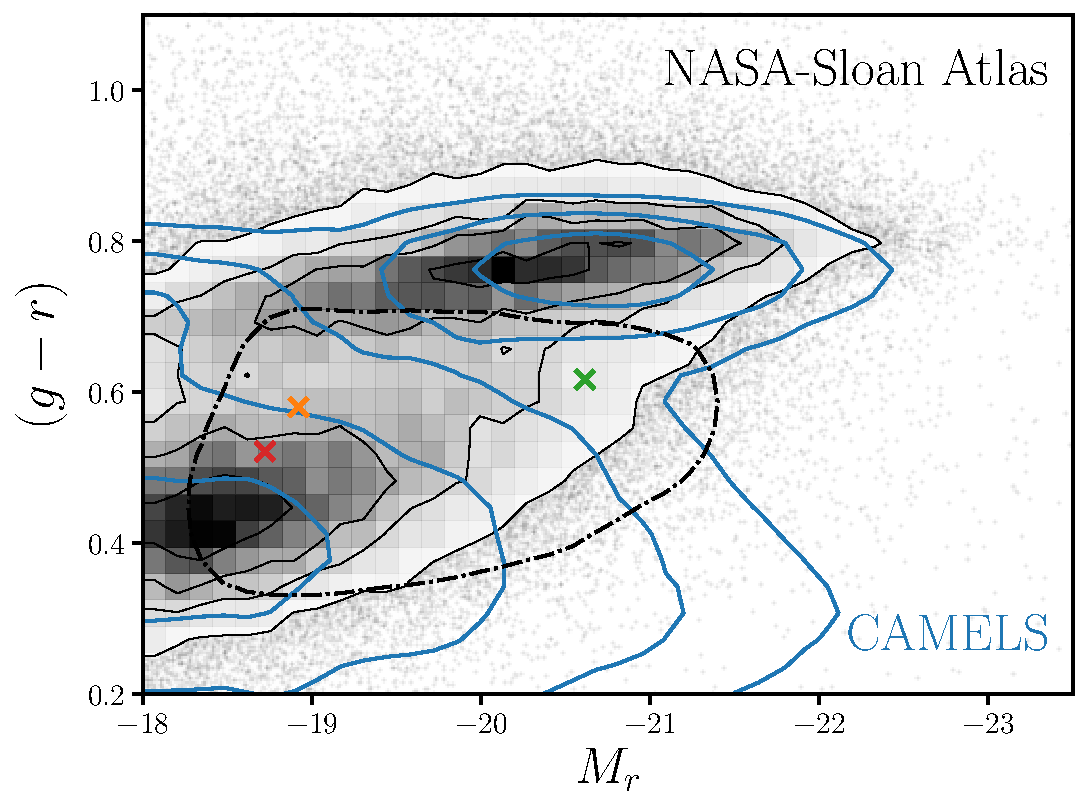
\includegraphics[width=0.9\columnwidth]{figs/nsa.pdf}} 
    \vskip -0.1in
    \caption{Color-magnitude distrubtion, $(g-r) - M_r$, of observed galaxies
    from the NSA (black) and simulated galaxies from CAMELS-TNG (blue). 
    Overall, the distributions of NSA and CAMELS-TNG galaxies are in good
    agreement. 
    The distribution for CAMELS-TNG is significantly broader since its simulated
    galaxies are generated using a wide range of cosmological and baryonic
    feedback parameters.
    }\label{fig:nsa}
\end{center}
\vskip -0.3in
\end{figure}

We use simulated galaxies from CAMELS, a suite of hydrodynamical
simulations constructed over a wide range of cosmological and
hydrodynamical parameters.
In particular, we use the 1,000 hydrodynamical simulations constructed using
the state-of-the-art IllustrisTNG model (CAMELS-TNG). 
The simulations are generated with different cosmological parameters,
$\Omega = \{\Omega_m, \sigma_8\}$, and baryonic feedback parameters, 
$\mathcal{B} = \{A_{\rm SN1}, A_{\rm SN2}, A_{\rm AGN1}, A_{\rm AGN2}\}$,
arranged in a latin hypercube. 
$A_{\rm SN1}$ and $A_{\rm SN2}$ represent the normalization factors for the 
galactic wind flux and speed; 
$A_{\rm AGN1}$ and $A_{\rm AGN2}$ represent the normalization factors for the 
energy output and specific energy of AGN feedback.
%All the cosmological parameter besides $\Omega_m$ and $\sigma_8$ are fixed: $\Omega_b = 0.049$, $h = 0.6711$, $n_s = 0.9624$, $\sum m_\nu = 0.0$eV, and $w = -1$.
%The CAMELS-TNG simulation all have a comoving volume of 
%(25 $h^{-1}{\rm Mpc}$)$^3$.
%They each evolve $256^3$ dark matter particles and $256^3$ fluid elements from
%$z=127$ to $z=0$ from initial conditions generated using second order
%perturbation theory. 
%Each simulation has 34 saved snapshots from $z=6$ to $z=0$. 
%Since we target $z < 0.05$ NSA galaxies, we only use the $z=0$ snapshot. 
%All the cosmological parameter besides $\Omega_m$ and $\sigma_8$ are fixed:
%$\Omega_b = 0.049$, $h = 0.6711$, $n_s = 0.9624$, $\sum m_\nu = 0.0$eV, and 
%$w = -1$.
%The SUBFIND~\citep{springel2001, dolag2009} algorithm is run on each simulation
%to identify halos and subhalos.
%SUBFIND computes physical quantities of the subhalos and the galaxies that
%resides in them. 
%For additional details on CAMELS, we refer readers to
%\cite{villaescusa-navarro2021, villaescusa-navarro2022a}.

In the 1,000 simulations, there are $\sim$700,000 galaxies with 
$M_* > 2\times10^8 M_\odot/h$. 
The galaxies, however, are not evenly distributed across them and have a
significant dependence on the parameters.  
For instance, simulations constructed at higher $\Omega_m$ values have more
galaxies.  
We correct for this implicit prior on the CAMELS parameters by randomly
selecting 100 galaxies from each simulation. 
This imposes a uniform prior: $p(\Omega, \mathcal{B}) = 1$ and leaves us with 
a total of 100,000 CAMELS-TNG galaxies.  

Since our aim is to analyze the observed photometry of NSA galaxies, we forward
model photometry for the simulated galaxies. 
CAMELS-TNG already provides synthetic dust attenuated stellar photometry for
each simulated galaxy~\citep{nelson2018}.
The unattenuated SED of a galaxy is computed by combining the SEDs of every
star particle of the host subhalo. 
Each SED is modeled as a single-burst simple stellar population using stellar
population synthesis (SPS) based on the recorded birth time, metallicity, and
mass. 
The SPS uses FSPS~\citep{conroy2009}, Padova isochrones, MILES
stellar library, and assumes a Chabrier initial mass function. 
The unattenuated galaxy SEDs are then attenuated using a dust model based on
the metal content of the neutral gas distribution in and around each
galaxy.
Afterwards, the SED is convolved with SDSS $g$, $r$, $i$, $z$-band photometric
bandpasses to produce the photometry: $X_i$. 
%For additional details on the synthetic photometry, we refer readers to \cite{nelson2018}. 

Next, we add noise to the synthetic photometry based on the measured
uncertainties, $\sigma_X$, of NSA galaxies. 
For each galaxy, we randomly sample $\sigma_{X,i}$ from the range of
uncertainties measured in NSA. 
Afterwards, we apply the uncertainty using a Gaussian with standard deviation
$\sigma_{X,i}$: $\hat{X}_i \sim \mathcal{N}(X_i, \sigma_{X, i})$. 
Although our noise model is simplistic, this is not an issue in our
approach beacuse the posteriors we ultimately evaluate are conditioned on the
uncertainties~\citep{hahn2022a}. 
In Fig.~\ref{fig:nsa}, we present the color-magnitude distribution of the
forward modeled CAMELS-TNG galaxies in blue. 
We reserve a random 10\% of these galaxies as a test dataset for validation
later Sec.~\ref{sec:valid}.
